\section{Kurzfristige Folgen}
\begin{frame}{Temperaturverlauf 1}
\begin{figure}
	\centering
	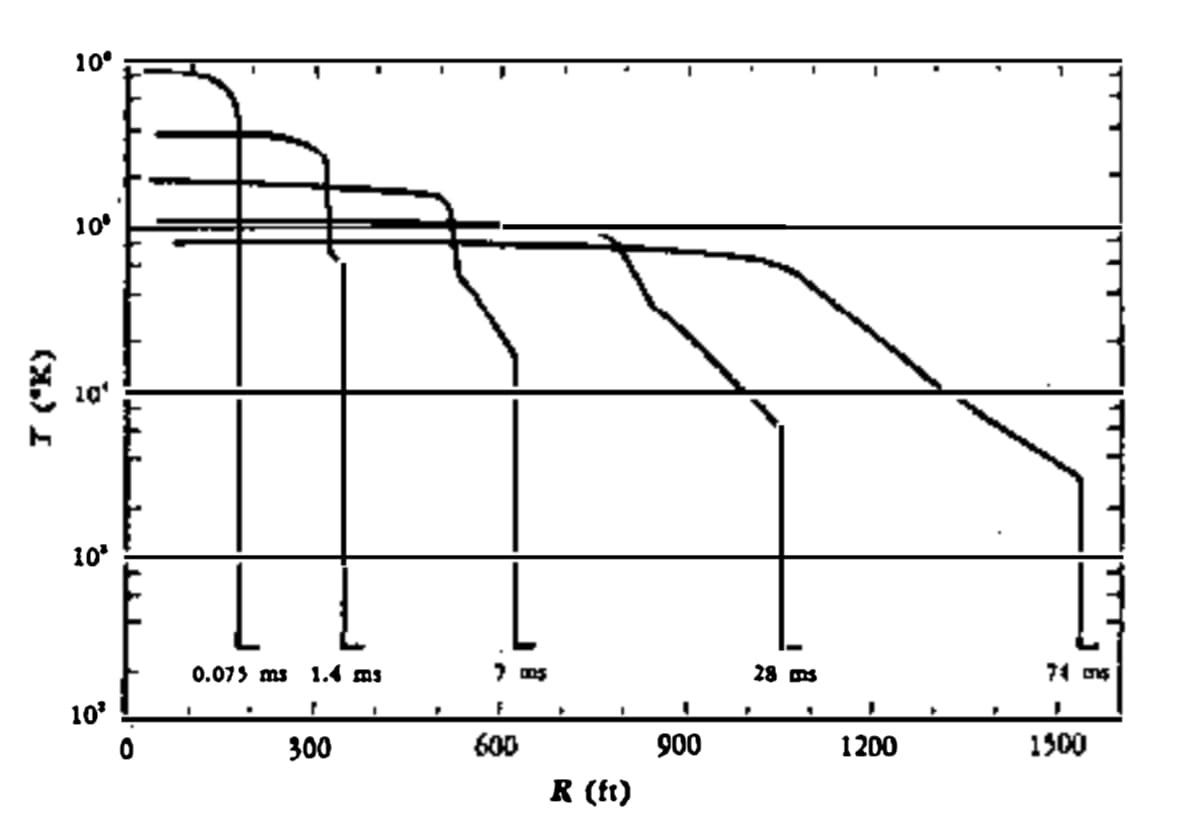
\includegraphics[width=0.5\linewidth]{img/img1}
	\caption{Temperaturen in Abhänigkeit der Entfernung für verschiedene kurze Zeiten nach einer Explosion der Energie $\SI{1}{\mega \tnt}$.\cite{AnnuRev18_1}}
\end{figure}
\end{frame}
\begin{frame}{Temperaturverlauf 2}
	\begin{figure}
		\centering
		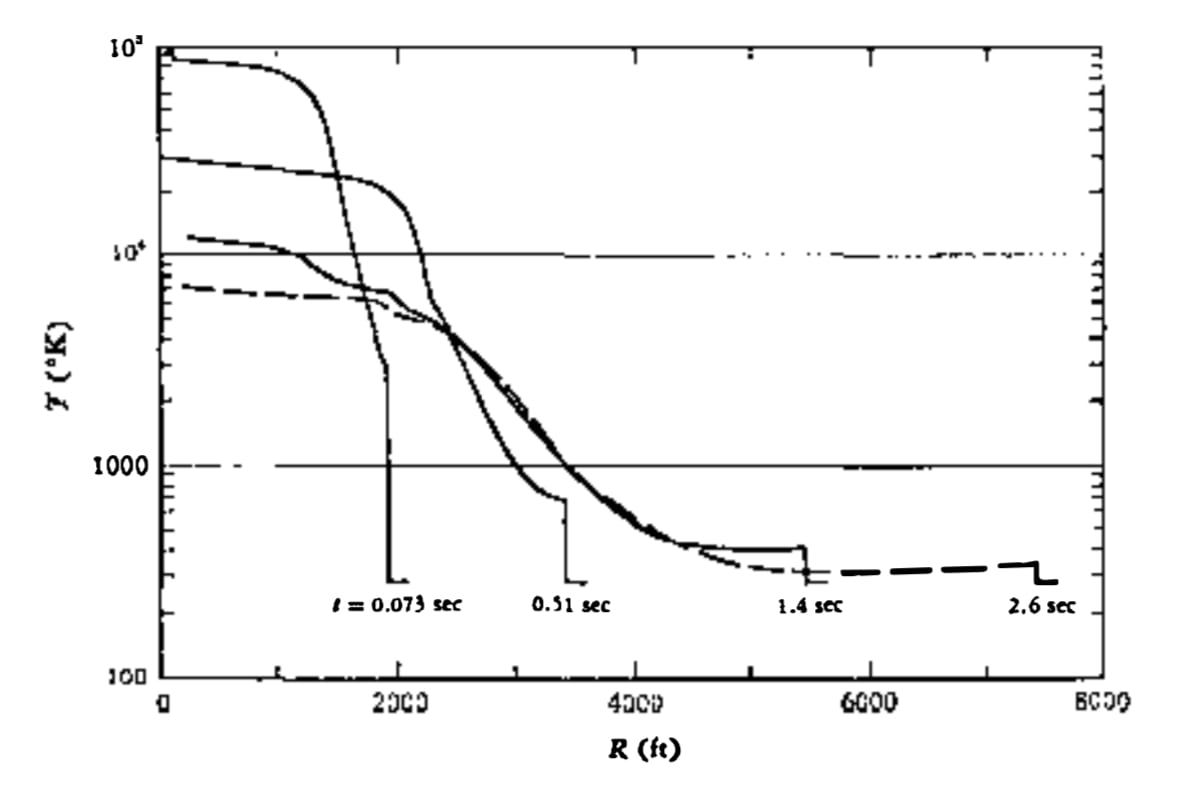
\includegraphics[width=0.5\linewidth]{img/img3.jpg}
		\caption{Temperaturen in Abhänigkeit der Entfernung für verschiedene längere Zeiten nach einer Explosion der Energie $\SI{1}{\mega \tnt}$.\cite{AnnuRev18_1}}
	\end{figure}
\end{frame}
\begin{frame}{Dichteverlauf}
	\begin{figure}
		\centering
		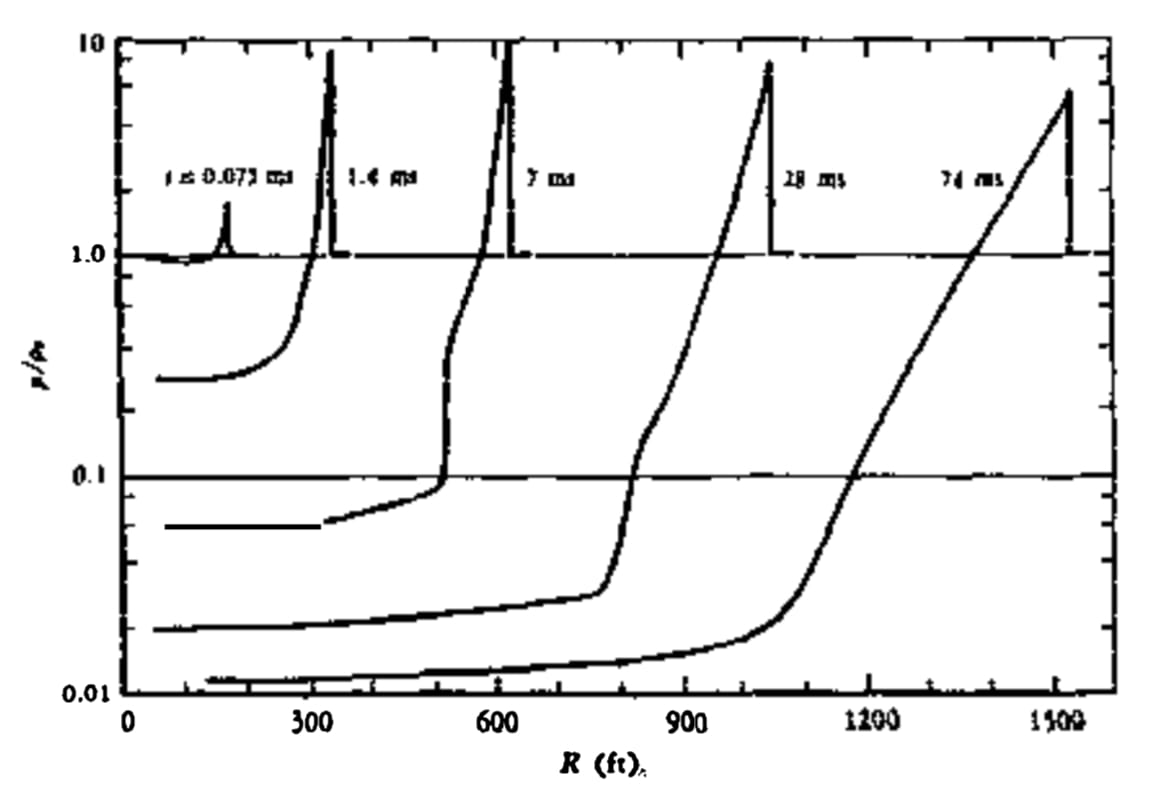
\includegraphics[width=0.5\linewidth]{img/img2.jpg}
		\caption{Luftdichte in Abhänigkeit der Entfernung für verschiedene Zeiten nach einer Explosion der Energie $\SI{1}{\mega \tnt}$.\cite{AnnuRev18_1}}
	\end{figure}
\end{frame}
\begin{frame}{Übersicht}
	\begin{itemize}
		\item starke Überdruckwelle, gefolgt von ebenfalls großer Unterdruckwelle
		\item gigantische Hitzeentwicklung
		\item vierstellige Temperaturen in Kilometern Entfernungen
	\end{itemize}
\end{frame}
